\documentclass[tikz,border=8pt]{standalone}
\usetikzlibrary{patterns,arrows.meta,calc}
\begin{document}
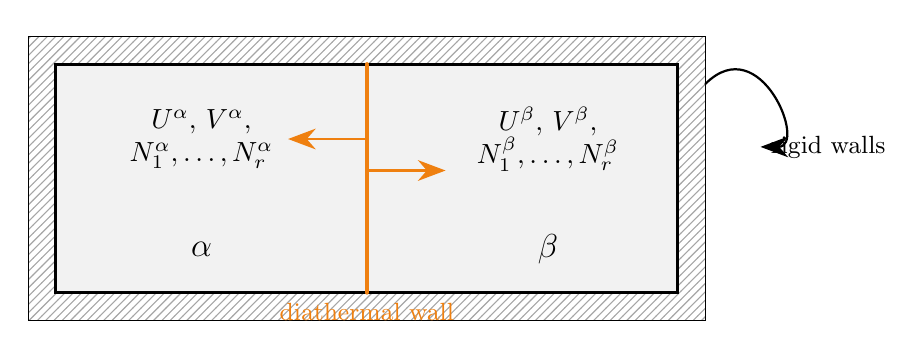
\begin{tikzpicture}[line cap=round]
  \tikzset{
    rigid/.style={pattern=north east lines, pattern color=gray!70},
    wall/.style={line width=1pt},
    label/.style={font=\small}
  }
  \colorlet{wallfill}{gray!10}

  % Outer rigid shell
  \draw[rigid] (0,0) rectangle (8.6,3.6);
  \fill[wallfill] (0.35,0.35) rectangle (8.25,3.25);
  \draw[wall] (0.35,0.35) rectangle (8.25,3.25);

  % Diathermal barrier
  \draw[line width=1.5pt,orange!75!brown] (4.3,0.35) -- (4.3,3.25);
  \node[font=\small,orange!75!brown] at (4.3,0.1) {diathermal wall};

  % Left subsystem
  \node[align=center] at (2.2,2.3) {$U^\alpha,\,V^\alpha,$ \\ $N_1^\alpha,\ldots,N_r^\alpha$};
  \node[font=\large] at (2.2,0.9) {$\alpha$};

  % Right subsystem
  \node[align=center] at (6.6,2.3) {$U^\beta,\,V^\beta,$ \\ $N_1^\beta,\ldots,N_r^\beta$};
  \node[font=\large] at (6.6,0.9) {$\beta$};

  % Heat-only arrows
  \draw[-{Stealth[length=10pt]},thick,orange!75!brown] (4.3,2.3) -- ++(-1.0,0.0);
  \draw[-{Stealth[length=10pt]},thick,orange!75!brown] (4.3,1.9) -- ++(1.0,0.0);

  % Rigid wall label
  \draw[-{Stealth[length=10pt]},thick]
    ($(8.6,3.0)$) .. controls +(0.7,0.7) and +(0.6,0) .. ($(9.3,2.2)$)
    node[right,label] {rigid walls};
\end{tikzpicture}
\end{document}
